\chapter{Centre Storage Management}
\label{chap:centre-storage-management}
Storage containers share common attributes, these attributes are grouped into
and defined in a \entitytarget{ContainerType}. Some storage containers hold
sub-containers, while others hold specimens.

A \entitylink{ContainerType} has the following attributes: a short name used
for quick identification; an optional description that gives more details for
the name; the \compfont{shared} flag used to share this container type with
other centres when assigned a \compfont{true} value; the \compfont{enabled}
flag used to allow containers of this type to be created when assigned a
\compfont{true} value.

A \entitytarget{StorageContainerType} is used to define the attributes for
containers that hold sub-containers. E.g. a freezer of certain dimensions holds
a number of racks, where each rack may hold many microwell plates. Figure
\ref{fig:centre-container-type} shows that a \entitylink{StorageContainerType}
is derived from \entitylink{ContainerType} and points to one or more child
container types. A storage container also has the attribute named
\compfont{topLevel} which is used to identify containers types that represent
the top of the hierarchy (e.g. a freezer).

A \entitytarget{SpecimenContainerType} is used to define the attributes for containers that only
hold specimens. E.g. a 96 well microwell plate is a type of specimen container that holds 96 tubes
where each tube contains a specimen. Microplates, where specimens are stored on the plate itself and
not in tubes held by the microwell, can also be managed by setting \compfont{isMicroplate} to
\compfont{true}. \entitylink{StorageContainerType} is also a subclass of
\entitylink{ContainerType}.

\begin{figure}[H]
  \centering
  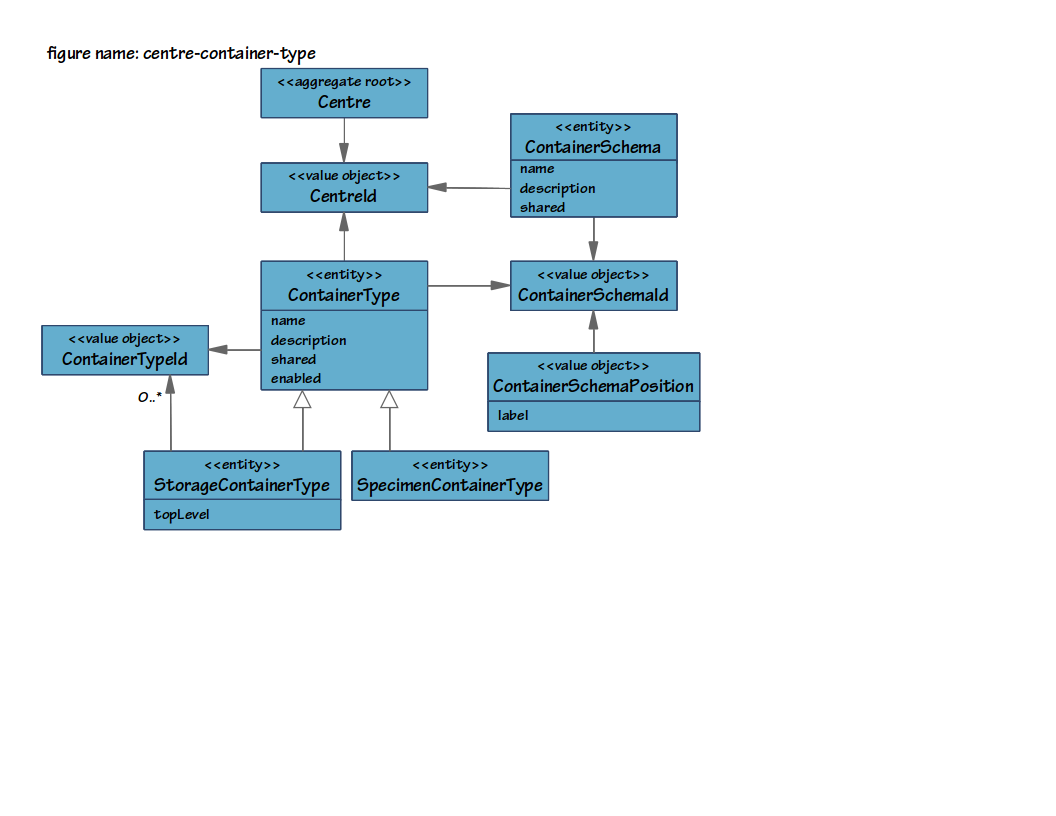
\includegraphics[trim={10mm 73mm 92mm 18mm}, clip,
    width=0.75\textwidth]{images/centre-container-type}
  \caption{Container Type model}
  \label{fig:centre-container-type}
\end{figure}

Each container type has a \entitytarget{ContainerSchema} that defines how the
sub-containers are \emph{labeled}. A label is a physical label that is stuck
onto a sub-container and is used to quickly identify it\footnote{This label
  identifies the position within the parent and does not include the parent's
  label. It is different than the label used by a container which includes the
  parent's label as a prefix.}. A container schema has multiple
\entitytarget{ContainerSchemaPosition}s which define the valid labels for the
container type (see Appendix \ref{appx:container-labeling} for more information
on how containers can be labelled). A single container schema may be used by
one more container types. Each container schema has a name for quick
identification and a description. The \compfont{shared} flag is used to share
the schema across different centres.

Figure \ref{fig:centre-container} shows the model used for containers. It is
described below.

\begin{figure}[H]
  \centering
  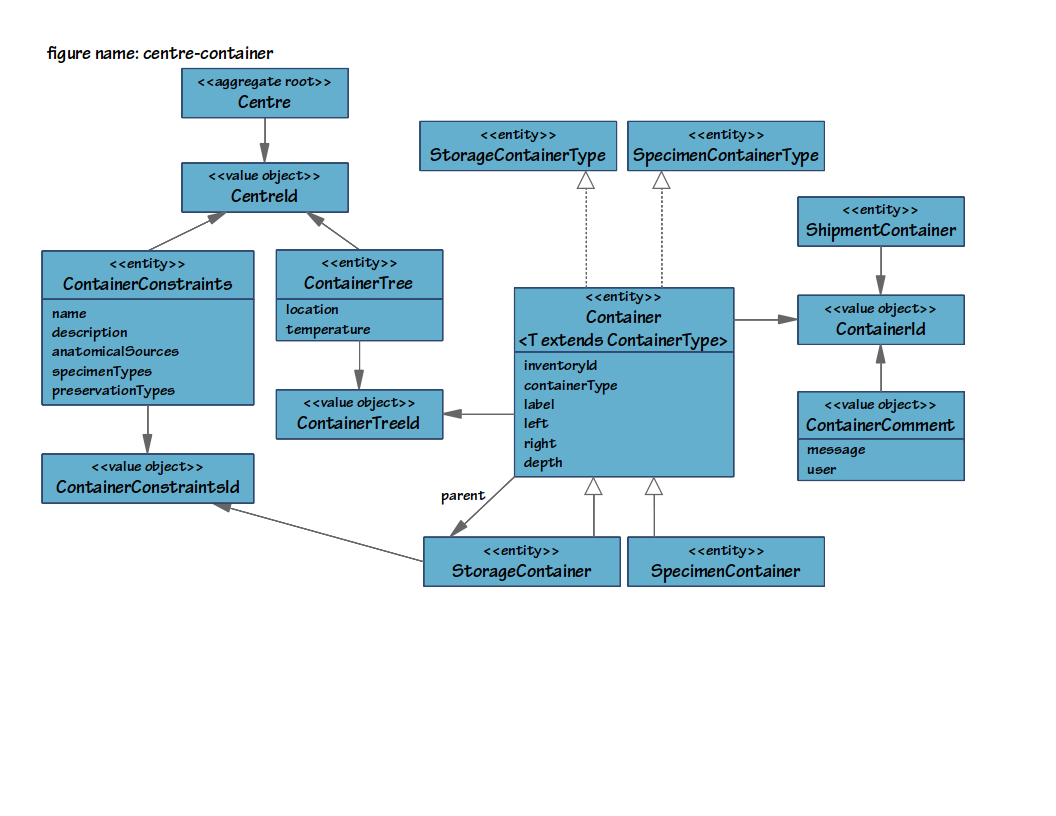
\includegraphics[trim={10mm 68mm 14mm 18mm}, clip,
    width=1\textwidth]{images/centre-container}
  \caption{Container model}
  \label{fig:centre-container}
\end{figure}

\subsection*{Container}
A \entitytarget{Container} is used to model physical containers used for
storage. The \entitylink{Container} class is a generic class with a type that
is either a \entitylink{StorageContainerType} or
\entitylink{SpecimenContainerType}. Two derived classes are available: either
\entitytarget{StorageContainer} or \entitytarget{SpecimenContainer}.

A \entitylink{Container} has the following attributes: an
\compfont{inventoryId} that is a unique identifier; the ID of it's container
type; the ID of it's parent container; the label which has the parent's label
as a prefix; the label within it's \entitylink{ContainerSchemaPosition}; and
the ID of the \entitylink{ContainerTree} it belongs to.

A \entitylink{ShipmentContainer} may reference a container using the
\valobjlink{ContainerId}. Comments can be attached to a container using
\entitytarget{ContainerComment}.

\subsection*{StorageContainer}
A \entitylink{StorageContainer} is a subclass of \entitylink{Container} and is
used to represent a physical container that holds sub-containers or specimen
containers. A storage container may have an optional
\entitylink{ContainerConstraint} to limit the types of specimens that it and
it's child containers may hold.

\subsection*{SpecimenContainer}
A \entitylink{SpecimenContainer} holds specimen tubes or other receptacles that
hold biological specimens.

\subsection*{ContainerTree}
A \entitylink{ContainerTree} holds attributes common to a whole container
hierarchy. It's attributes are: the center ID of the center it belongs to; and
the center's location (in the case a center has multiple locations).

\subsection*{ContainerSchemaPosition}
\entitytarget{ContainerSchemaPosition} tracks the label position within the
parent that this container holds. Only one container can be linked with a
schema position.

\subsection*{ContainerConstraint}
As shown in Figure \ref{fig:container-constraint}, an optional
\entitylink{ContainerConstraint} can be used with a storage container to limit
the specimens that it and it's child containers can hold. A container
constraint has the following attributes: a short identifying name; an optional
description; the allowed anatomical sources; the allowed specimen types; and
the allowed preservation types. A container constraint entity is assigned to a
centre and a centre location, and then containers of that center can use the
constraint.

\begin{figure}[H]
  \centering
  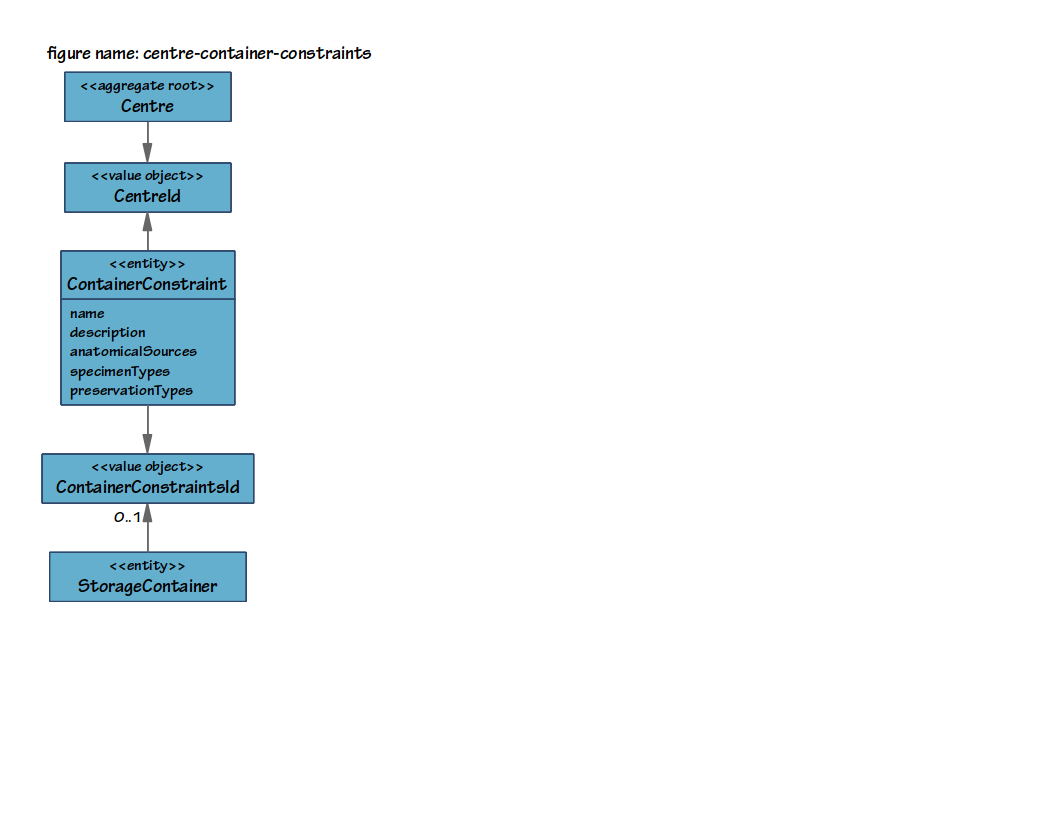
\includegraphics[trim={10mm 54mm 212mm 18mm}, clip,
    width=0.25\textwidth]{images/centre-container-constraint}
  \caption{Container constraints}
  \label{fig:container-constraint}
\end{figure}

% Local Variables:
% compile-command: "/usr/bin/rubber --pdf main"
% End:
